%===================================== CHAP 4 =================================

\chapter{Research Method}\label{chap:4}

The purpose of this project is to create a prototype to improve student's motivation for applying for exchange program by recommending courses and universities. The research questions were first created after defining the purpose and refined after identifying the background, motivation, relevant theory and related work through literature review, as according to Oates' model \cite{oates2005researching} of the research process. The research questions were answered by evaluating a prototype created by using the design and creation strategy. The final evaluation was done by using primarily quantitative data analysis on data generated by questionnaires and an offline experiment.

The Oates'\cite{oates2005researching} model of the research process was used as a guideline for selecting the research methods that could best answer the research questions. The model and the specific methods chosen is displayed in Figure \ref{fig:research_process}. This chapter is structured after Oates' model. First, the chosen research strategy is presented. Next, the data generation methods are described with their respective ways to analyze the data they produce. The ethical issues are then detailed to ensure that the rights and dignity of the research participants are maintained. Finally, the practical issues that could impact and limit the research project are discussed. 

\begin{figure}[H]
    \centering
    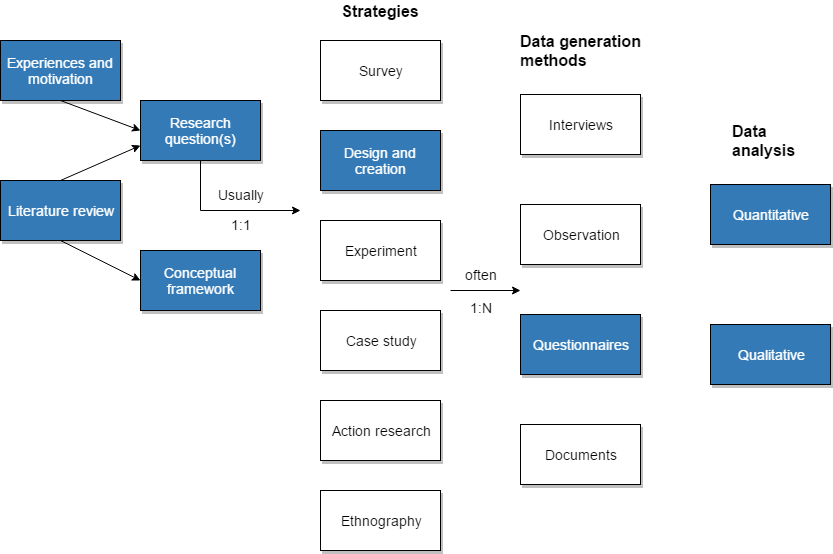
\includegraphics[width=1\textwidth]{fig/research_process.png}
    \caption{The outlined research process}
    \label{fig:research_process}
\end{figure}



\section{Research Strategy: Design and Creation}

This project used the design and creation strategy to develop a computer-based artefact named Utsida. Utsida is a prototype that was utilized as a tool to answer the research questions detailed in section \ref{RQ}.   

Utsida consists of two sub-systems, a case-based reasoning recommender system (CBR-RS) and a web application for user interaction and data storage. Utsida was used as a tool to generate the data needed to answer both RQ1 and RQ2. The CBR-RS incorporated the AI methodology CBR to enable a new way of recommending relevant universities and courses for an exchange program. The web application part used the CBR-RS to give recommendations and included the features of the requirement list (section \ref{sec:requirements}) to have an affect on student motivation and answer RQ1.

To answer RQ1, the system needed to be well functioning and easy to use. Therefore it was beneficial to use the design and creation strategy to assist with the development of the system. The design and creation was done in an iterative process according to the five steps from Vaishnavi and Kuechler \cite{vaishnavi2004design}: Awareness, Suggestion, Development, Evaluation, and Conclusion.

\subsection{Awareness and Suggestion}

The awareness step involves finding and defining the problem domain. Gaining awareness was done in the preliminary research (Chapter \ref{chap:2}) and through the production of research questions (section \ref{RQ}). When the problem had been identified, a suggestion for the system was made (Chapter \ref{ch5:implementation}). This suggestion included the first design details of the system which initiated the development process. The awareness step was also performed throughout the development process, typically after usability tests or user evaluations. 

\subsection{Development}

To answer the research questions it was necessary to produce data on user interaction and satisfaction. It was, therefore, essential that the web application part of Utsida was easy and intuitive to use. To ensure high user satisfaction, the development of Utsida was conducted in an iterative manner. This included communicating with potential users throughout the development and conducting usability tests. The spiral model, introduced by B. W. Boehm \cite{boehm1988spiral}, is a common model for iterative development, and was chosen as the foundation for the development process of Utsida. Each spiral in the model includes steps for analyzing risks and requirements, development and testing of a prototype, planning the next iteration, and determining the objective of the next iteration. The model was modified to the needs of the study. Figure \ref{fig:development_process} displays the modified version of the spiral model, where the main differences are less risk assessment, verification, and validation of each prototype. The changes were done to be able to quickly try out new functionality, ideas, and get them tested to see if they are feasible. Furthermore, as this was a relatively short-term study, there was limited time available for analysis and validation of each cycle.

\begin{figure}[h]
    \centering
    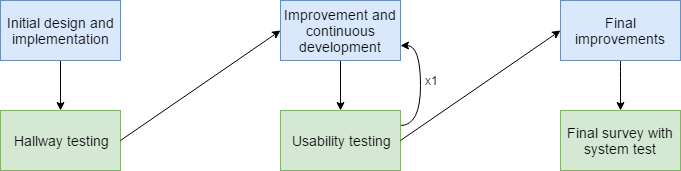
\includegraphics[width=1\textwidth]{fig/development_process.png}
    \caption{The development process of Utsida}
    \label{fig:development_process}
\end{figure}

\subsection{Evaluation and Conclusion}

Evaluation was done continuously after each development cycle and the whole process was redone if found needed. Part of the iterative evaluation was done by testing the system on students through usability tests and hallway testing. The final evaluation was done through an online test with an accompanying questionnaire, an offline experiment, and by analyzing data on motivational factors. These data generation methods are detailed further in section \ref{sec:questionnaire_1}, \ref{sec:questionnaire_2} and \ref{sec:observation_test}.

\subsubsection{Usability Testing}

Iterative sessions of usability testing were performed on the web application to evaluate and ensure sufficient usability. The test participants were selected and consisted in a large degree of students who had an understanding of the current approach for applying for an exchange program. Students from different programs was tested to ensure a broad specter of backgrounds. These tests helped find flaws in both general functionality and design so that the system was as reliable as possible before conducting the final online test. Data was be gathered by interviewing the testers, observing their use of the system, and have them fill out a System Usability Scale (SUS)-schema \cite{brooke1996sus}. After each test, the data was be analyzed using the SUS score \cite{brooke1996sus}.

\section{Data Generation Methods}
Because there was no client or persons with high stakes in this study, interviews were not viewed upon as a feasible method to generate data. Data generation through documents were also not viable because of no existing documents about the problem context. However, questionnaires and experiments are standard methods to produce data about a software system \cite{oates2005researching}, and suited the study's need of obtaining generalized opinions about the system's effect and functionality. They were therefore chosen as the designated data generation methods. 

\subsection{Questionnaires}

Two questionnaires were used to produce data to answer the research questions. The first, questionnaire 1, was conducted during the development of the system with the goal of learning what students think are the most important motivational factors for choosing an exchange location, see section \ref{sec:questionnaire_1} for further details. The second, questionnaire 2, was conducted after the system prototype was completed, as a final evaluation and user test of Utsida. All the details of the second questionnaire can be found in section \ref{sec:questionnaire_2}.

Both questionnaires were self-administrated, which promoted the opportunity to collect data from a representative number of students at once. This method also suited the limitations of this project well with low cost and reduced time usage for conducting and planning the test compared to administrated tests. The recipients of the questionnaire will be students who have some experience with exchange studies. To acquire a larger target group who fits this criterion, the OIR will be contacted for possible access to email lists and Facebook sites.

The majority of the questions in the questionnaires was closed questions. The form of the questions in the questionnaires were Likert scale \cite{allen2007likert}, semantic differential scale \cite{osgood1952nature} and questions with \enquote{Yes}, \enquote{No}, or \enquote{Don't know} options. According to Dawes J. G. \cite{dawes2012data}, the results from using a 5-point- and 7-point scale are very similar. Questionnaire 1 will use a 7-point scale, while questionnaire 2 will use a 5-point scale. A 7-point scale was chosen to better fit the model in MyCBR Workbench where the weights are represented in a range from 1-10. A 5-point scale, however, was selected to describe the degree of agreement on the statements in questionnaire 2. It also suited well with the possible answers (Figure \ref{fig:q2_question_form}). Also, the students was asked optional open questions where they could articulate their opinions.

\subsubsection{Validity and Reliability}
Content validity is concerned with whether the questions in the questionnaire represents a good sample of actual problem to be investigated \cite{oates2005researching}. The means that the selected questions should cover all the different evaluations needed to answer the research questions accurately. Feedback from potential participants and experts were used to evaluate the validity. For RQ2 the central aspect is the \enquote{suitability} and whether the system recommends viable universities and courses. RQ1 concerns the effect on the motivation of the students, and here the most critical evaluations is the use of the system, motivational effect and recommendation to others.

Construct validity means that the questionnaire is evaluating what it was intended to evaluated and not other aspects \cite{oates2005researching}. Questionnaire 1 and 2 were designed to ensure the construct validity by using clear and straightforward questions that targeted the specific dimensions of the research questions. An iterative process was followed in the design of the questionnaire to remove or edit possible irrelevant and poorly formulated questions. 

The measurement of reliability is that the questionnaire yields the same result when given to the participants repeatedly. The reliability is hard to assess as the questionnaire was given only once to participants, and the participants do not evaluate the system over time. Evaluating the system over time with part of participants would also have distorted the data by giving them more time to be familiar with the system. However, one way to measure the reliability of the internal consistency is using Cronbach's alpha \cite{bland1997statistics}.

\subsubsection{Bias}

By using questionnaires as the primary method to collect data, several risks of bias were introduced. The majority of the questions were, therefore, striven to be neutral statements which the participants can state their degree of agreement as given by the Likert scale \cite{allen2007likert}. Furthermore, the target population for the questionnaires were students who are interested in exchange in some way, which might influence responses to be more positive. 

Central tendency bias is a risk when the questions have extreme response categories, this is especially relevant for the Likert scale and Semantic Differential Scale. This means a participant will more often answer in the middle of the scale. A lower point scale will be used in questionnaire 2 to reduce the central tendency, and both questionnaires will have precise questions that reduce the confusion of the participants and their likelihood of answering in the middle values of the scale. 

Acquiescence bias is when the participant is likely to answer positively on a question \cite{cronbach1946response}. To reduce the acquiescence bias, the questions avoided being strongly positively based. However due to the nature of the questions having less social desirability and not being sensitive an acquiescence bias were less likely to have a large impact.  This is similar for social desirability biases.  

Considering the expected response rate was a small proportion of the full population, non-response bias is unavoidable. There could always be a general difference between the opinions of those who choose to answer the questionnaire and those who do not. Those who did not participate might think the research sounds uninteresting, and if they participated, they might respond with more negative answers. Non-response bias will be taken into consideration when discussing the final result data in Chapter \ref{ch:results&discussion}: Results & Discussion.



\subsection{Questionnaire 1: Motivational Factors}\label{sec:questionnaire_1}

The goal of questionnaire 1 was to gain knowledge on important factors for students when they choose an exchange location and university. The results from this questionnaire was the basis for the weighting of the attributes in the CBR-RS and choosing which attributes to include in the system. The target population was all Norwegian students that have either been on exchange or is considering going on exchange. This means that they had some background and considerations about their motivational factors. The total population size of questionnaire 1 is difficult to specifically estimate since it also includes students that are considering going on exchange. However the goal of the sample size was 100 students to ensure some variability in the answers. A higher sample size was believed to be difficult to obtain due to limitations in funds, time and access to publication sources for the questionnaire. 

%Skriv om statistic significance, confidence interval osv

The main question in questionnaire 1 was a closed question and it was formed according the semantic differential scale, see figure \ref{fig:semantic_scale}. The participant ranked each motivational factor according to the particular decisiveness of that factor. See appendix \ref{app:questionnaire1} for all the questions included in questionnaire 1. 

\begin{figure}[h!]
    \centering
    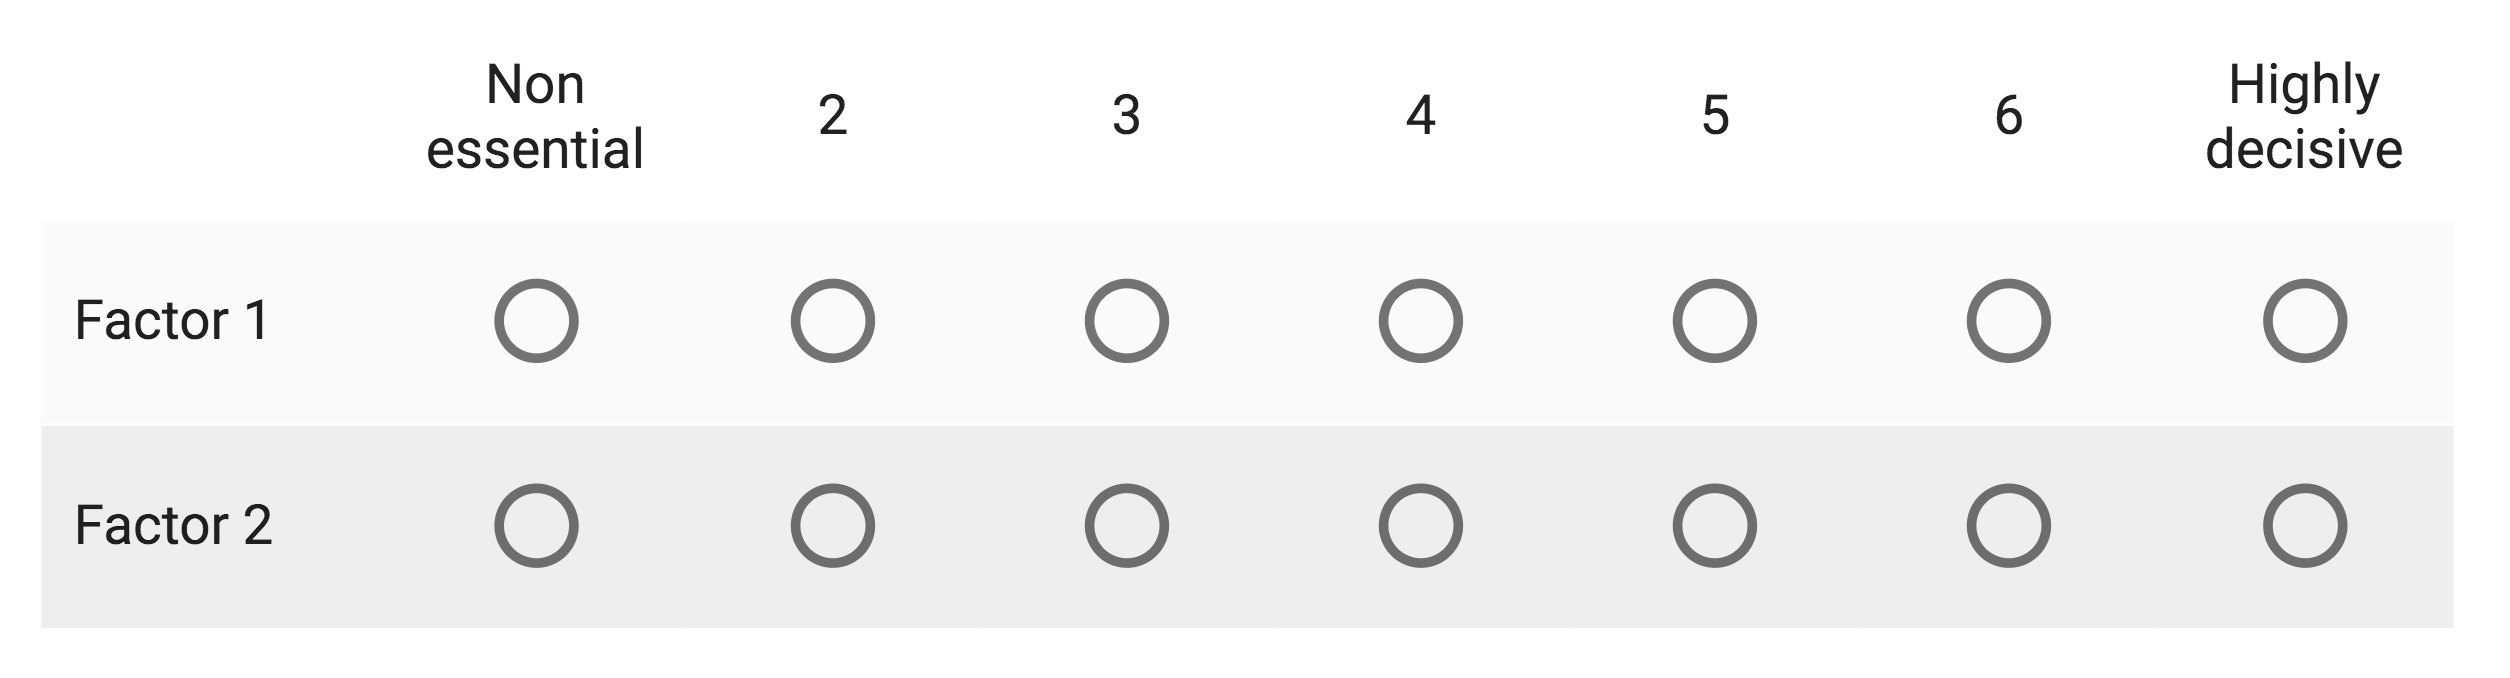
\includegraphics[width=1\textwidth]{fig/question1.png}
    \caption{The questionform in questionnaire 1}
    \label{fig:semantic_scale}
\end{figure}

This questionnaire also included an open ended question asking the students for feedback on possible other motivational factors that could be included in the system.

\subsubsection{Data analysis}
The numerical data from the questionnaire was analyzed in a quantitative manner, by calculating the mean, standard deviation and coefficient of variation for each attribute. The coefficient of variation was calculated to show the spread relative to the mean of the data and to rank each attribute against each other for the weighting purposes. Even though the data was originally ordinal was analyzed as interval data to better fit with the weighting in the CBR model. 

The open ended text question was analyzed in a qualitative manner by using theme analysis. First each question was reduced to only include important sections related to the goal of the question. All unrelated parts of text was be removed. Each answer was then analyzed by finding related themes of answers and mapping them in a table. The number of occurrences of a theme was then be counted and each theme ranked by importance. 

\subsection{Questionnaire 2: User Testing of Utsida}\label{sec:questionnaire_2}

The three goals of questionnaire 2 was to; 1. Evaluate and analyze how Utsida affects students motivation for applying for an exchange program, 2. Find out whether students who have already been on an exchange program thinks this system would make their process easier, and 3. Evaluate if the system delivered relevant recommendations to the user.

In order to keep the margin of error to a minimum it was important to get feedback from as many students as possible. According to the Norwegian Centre for Research Data \cite{utvekslingsopphold}, 3192 students at NTNU did an exchange program in 2016. The amount of students at NTNU who are interested in study exchange is hard to estimate, but the total target population for the questionnaire was set to 10000. The questionnaire was published through social media, and a cooperation was made with the OIR to publish it on their Facebook page with approximately 3300 followers- all being in the target group of this study. According to Krejcie \& Morgan \cite{krejcie1970determining} a sample size between 300 to 370 is optimal with a population size between 1400 and 10000, and therefore also optimal in this study. Considering the limitations of budget, time and that the main questionnaire included a lengthy user test, the expected sample size was considerably lower than the optimal size. Hence, a realistic goal of 60 participants was set.

The questionnaire consisted of two main parts of questions; one for reviewing the motivation and use of the application, and one for evaluation of CBR-RS' recommendations.

%Spørsmålsform, målgruppe, mål, hvordan det skal bli gjennomført, publiseringsmetoder, innsamling, data simplifisering?

\subsubsection{Part 1: Motivation and Use}
The questions in the first part were on a Likert-type form \cite{likert1932technique}. This question form is designed as a five-point scale where each option represents a degree of agreement to a given statement. This way, the questions can be neutral statements, where the recipients of the questionnaire could select their the level of agreement they relate to the most, leaving as little room for bias as possible. 

\begin{figure}[H]
    \centering
    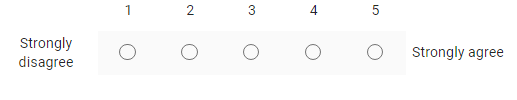
\includegraphics[width=1\textwidth]{fig/q2_question_form.PNG}
    \caption{The question form used in the first part of the questionnaire. Each question is lead by a statement regarding motivation.}
    \label{fig:q2_question_form}
\end{figure}

The questions in the first part of questionnaire 2 was targeted to find out what effect Utsida may have on the students motivation to apply for an exchange program. The students were presented with slightly different questions depending on whether they had participated in an exchange program or not.

\subsubsection{Part 2: Evaluation of Recommendation}

The second part of the questionnaire focused on the students evaluating the recommendations they receive from Utsida, as well as evaluating the results from two pre-defined queries to the CBR-RS. The question form was designed to have simple \enquote{Yes}, \enquote{No}, \enquote{Don't know} answers to easier determine the amount of students that received relevant recommendations. The pre-defined query recommendations also included a question which asked the students to rate the recommendations (see Figure \ref{fig:q2_rate_search}). The pre-defined queries, see Appendix \ref{pre_defined_search_table}, were included to evaluate the recommendations for a specific search that does did not rely on user input, and thus yielded objective evaluation. 

\begin{figure}[H]
    \centering
    
\includegraphics[width=1\textwidth]{fig/rate_search.png}
    \caption{Question form on the suitability of a pre-defined search}
    \label{fig:q2_rate_search}
\end{figure}


\subsubsection{Data analysis}
The data analysis on questionnaire 2 was done similar to questionnaire 1 by using quantitative analysis on the closed questions and simple qualitative analysis on the open-ended question. The closed questions likert scale was analyzed by the use of mode and frequencies. On the \enquote{Yes}, \enquote{No} or \enquote{Don't know} questions however, only percentages and number of answers for each option is presented. Cronbach's alpha was used to asses the internal consistency of the likert scale questions regarding motivation. 

\subsection{Offline experiment of Recommender System}\label{sec:observation_test}
An offline experiment method introduced by Ricci et al. \cite{ricci2011introduction} was used to evaluate the relevancy of the recommendations of the CBR-RS. This is a specific method to evaluate recommendation systems in an offline setting without user influence, and should not be misinterpreted as the \textit{Experiment} research strategy.

The offline experiment was conducted with 20 queries that were generated to simulate 20 unique users using the system (see Appendix \ref{app:user_queries}). Each query was sent sent to two different CBR-RS models. One with adjusted similarity measures, taxonomies and weights, and one with a standard exact match search. The scores for each outputting recommendation was then given according to the score metric in Table \ref{tab:offline_test} and the total score for each model was the sum of the means. The hypothesis was that the relevancy of the model with adjusted similarity would score higher than the model with a simple full match search. 

This method was beneficial to test the CBR-RS with a large set of possible inputs but with a low cost. One common downside is that the queries only represent a small part of the possible user searches. To mitigate this the queries were selected to cover a wide range of attributes and users with different backgrounds. Another disadvantage was that the offline experiment did not evaluate the recommender with actual users, this was however mitigated with continuous usability tests and questionnaire 2.


\begin{table}[h]
\centering
\resizebox{\textwidth}{!}{%
\begin{tabular}{|
>{\columncolor[HTML]{D0E0E3}}l |l|l|l|}
\hline
\multicolumn{4}{|c|}{\cellcolor[HTML]{A4C2F4}{\color[HTML]{333333} Rating scale for recommendations (0-10 points)}}                                                                                             \\ \hline
Attribute           & \cellcolor[HTML]{D0E0E3}0 points                                         & \cellcolor[HTML]{D0E0E3}1 point                                             & \cellcolor[HTML]{D0E0E3}2 points \\ \hline
Institute           & \begin{tabular}[c]{@{}l@{}}Wrong faculty \\ wrong institute\end{tabular} & \begin{tabular}[c]{@{}l@{}}Correct faculty\\ wrong institute\end{tabular}   & Correct Institute                \\ \hline
Year                & Before 2011                                                              & 2011-2013                                                                   & 2014-2017                        \\ \hline
Geographic Location & \begin{tabular}[c]{@{}l@{}}Wrong country \\ wrong continent\end{tabular} & \begin{tabular}[c]{@{}l@{}}Correct continent\\ wrong country\end{tabular}   & Correct country                  \\ \hline
University          & \multicolumn{2}{c|}{No match}                                                                                                                          & Perfect match                    \\ \hline
Language            & No match                                                                 & \begin{tabular}[c]{@{}l@{}}The language is \\ part of the list\end{tabular} & Perfect match                    \\ \hline
Ratings             & \multicolumn{3}{c|}{0.5 points for each rating in range (-1, rating +1)}                                                                                                                  \\ \hline
\end{tabular}%
}
\caption{Score matrix for offline observation test}
\label{tab:offline_test}
\end{table}

\subsubsection{Data Analysis}
The offline experiment generated quantitative data that was statistically analyzed. The central tendency were analyzed with the mean and standard deviation measures, and paired t-test were conducted to define the significance of the result. The confidence level was 95\% with a p-value limit of 0.05.

\section{Ethical Issues}
Some ethical issues regarding data collection and storage were considered in this study. The designated data collection methods kept all participants anonymous, but some meta-data was collected, such as which faculty and university they belong to. Furthermore, as an incentive for students to answer the questionnaires, lottery prizes were promoted for participating. To be able to enter the lottery, the participants had to enter their e-mail. This step was entirely optional. When each questionnaire was closed, the answers were stored in a Google Spreadsheet anonymously, and the entered e-mails were scrambled in a random order so that they were not linked to their answers. This way, there was no way to identify each answer. After the lottery was completed the emails were deleted and only the winner contacted. 

Informed consent was maintained in the questionnaires by informing the participants about the purpose and goals for the questionnaires, and by stating that the entire process for all participants is entirely voluntarily and that they can stop any time they want.

During the online test of the system, the users created an account which included storing their chosen password, e-mail, name and institute at NTNU. This information could not be linked to the questionnaire they took, but it still raised an ethical issue, considering the authors had access to this data. During the development of the system, steps were taken to ensure the confidentiality of the users of the system by using encryption and proper security measures.


\section{Practical Issues}
This study was performed by two students, with one advisor to guide the project. There was a limited amount of monetary funds, and the available time was only nine months. The data which served as the results was primarily produced by real users. With the minimal budget, a practical issue was to produce incentive for enough students to answer the surveys. Furthermore, because of the limited time, both larger administrated tests and self-administrated tests were considered out of reach.

\cleardoublepage